\documentclass{standalone}

\usepackage{pgfplots}

\begin{document}

    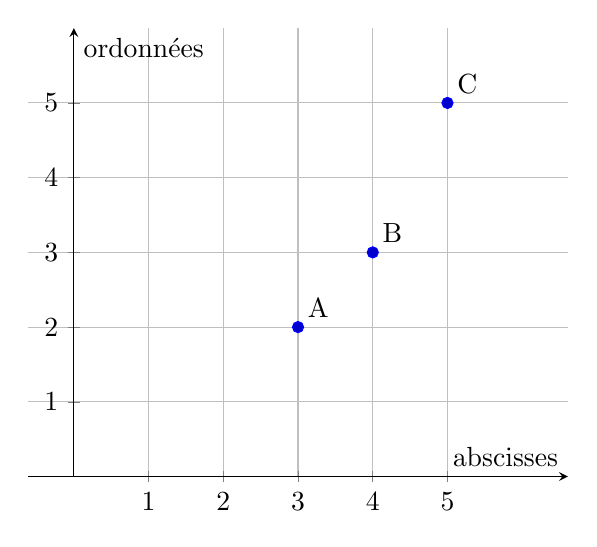
\begin{tikzpicture}
        \begin{axis}[axis lines=middle,
                    xlabel={abscisses},
                    ylabel={ordonnées},
                    xmin=0,
                    xmax=6,
                    ymin=0,
                    ymax=6,
                    xtick={0, 1,...,5},
                    ytick={0, 1,...,5},
                    axis equal,
                    grid=both]
            \addplot+[only marks] coordinates {(3, 2) (4,3) (5,5)};

            \node[above right] at (axis cs:3,2) {A};
            \node[above right] at (axis cs:4,3) {B};
            \node[above right] at (axis cs:5,5) {C};
        \end{axis}

    \end{tikzpicture}

\end{document}